\documentclass[12pt]{article}

\usepackage[margin=1in,footskip=0.25in]{geometry}
\usepackage{graphicx}

\begin{document}
	\underline{\LARGE{\centerline{Nikita Jagyasi}}}\\
	\\
	58, \rightline{Contact:8793477680}\\
	Old Subedar  \rightline{e-mail: jagyasinm@rknec.edu}\\
	Layout Extention, \\
	Nagpur - 440024	\begin{figure}[h]
		\hfill
		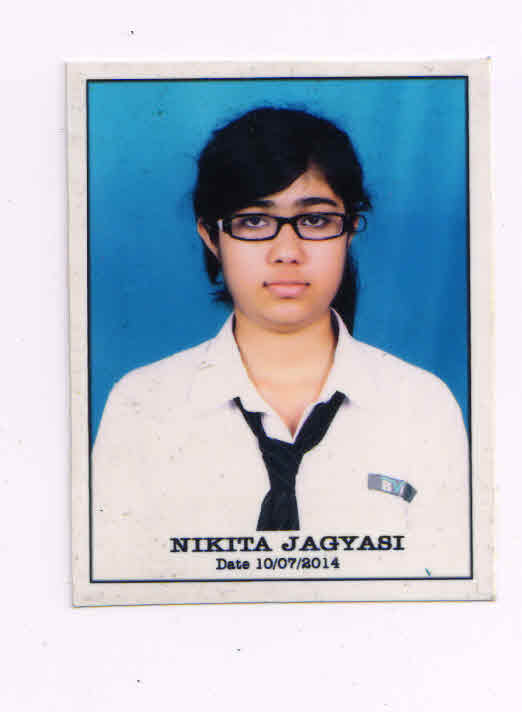
\includegraphics[height=2.5cm]{pic}
	\end{figure}\\
	\textbf{\textsc{OBJECTIVE : }}To work with an organization that will give me an opportunity to learn and grow along with the organization.\\
	\\
	\textbf{\textsc{EDUCATION : }}\\
	\\
	\begin{tabular}{|r|l|l|l|c|l|}
		\hline
		Sr No. & Degree & Institution & Board & Passing Year & Score\\
		\hline
		1. & 3\textsuperscript{rd} year & RCOEM & Nagpur University & 2018 & Pursuing\\
		2. & 2\textsuperscript{nd} year & RCOEM & Nagpur University & 2017 & CGPA 9.46\\
		3. & 1\textsuperscript{st} year & RCOEM & Nagpur University & 2016 & CGPA 9.46\\
		4. & 12\textsuperscript{th} & Bhavan's B.P. Vidya Mandir & CBSE & 2016 & 90\%\\
		5. & 10\textsuperscript{th} & Sanjuba High School & CBSE & 2014 & 95.2\%\\
		\hline
	\end{tabular}
		\\
	\\
	\\
	\textbf{\textsc{PROJECTS : }}
	\begin{enumerate}
		\item IOT based security system with e-mail alerts using PIR sensor and Raspberry Pi
		\item IOT based project that uploads DHT sensor data to a server like ThingsBoard
		\item Persistence of Vision Display using 8051 Microcontroller
		\item Distance measurement using Arduino
		\item Bank Management Project using C++ using File Handling and Database Management
	\end{enumerate}
	\textbf{\textsc{TRAINING \& INTERNSHIP : }}
	\begin{itemize}
		\item Training on Basic and Advanced Programming in C and C++ on Internshala
	\end{itemize}
	\textbf{\textsc{RESEARCH PUBLICATIONS : }}
	\begin{enumerate}
		\item None
	\end{enumerate}
	\textbf{\textsc{TECHNICAL SKILLS : }}
	\begin{itemize}
		\item C(intermediate)
		\item C++(intermediate)
		\item Python(intermediate)
		\item Linux(beginner)
		\item ROS(beginner)
		\item Assembly Language Programming for 8085 microprocessor and 8051 microcontroller
	\end{itemize}
	\textbf{\textsc{SOFT SKILLS : }}
	\begin{enumerate}
		\item Communication Skills
		\item Good Learning Skills
		\item Time Management Abilities
		\item Teamwork
		\item Multitasker
	\end{enumerate}
	\textbf{\textsc{EXTRA CURRICULAR ACTIVITIES : }}
	\begin{itemize}
		\item Dancing
		\item Was a part of organizing committee of events such as Personna, Minute to win it, organized under Pratishruti(our cultural fest)
		\item Was head girl of my school
	\end{itemize}
	\textbf{\textsc{CO-CURRICULAR ACTIVITIES : }}
	\begin{enumerate}
		\item Part of Robotics Club of college
		\item Was a part of organizing committee of TechQuiz, an event organized under Technovision(our technical fest)
	\end{enumerate}
	\textbf{\textsc{PERSONAL INFORMATION : }}\\
	\\
	\textsc{Father : }Manoj Hariram Jagyasi\\
	\textsc{Mother : }Rashmi Manoj Jagyasi\\
	\textsc{Date of Birth : }7\textsuperscript{th} August, 1998\\
	\textsc{Languages Known : }English, Hindi, Sindhi, Marathi\\
	\textsc{Alternate e-mail address : }nikitajagyasi@gmail.com\\
	\\
	\textbf{\textsc{REFERENCES : }}\\
	\\
	Dr. Rajesh Raut, Head of Department, e-mail : hodec@rknec.edu\\
	Prof. Deepak Khushalani, Embedded Systems Teacher, e-mail : khushalanidg@rknec.edu\\
	Akshay Marwadkar, Friend/Classmate, e-mail : marwadkarap@rknec.edu\\
	\\
\end{document}